%!TEX root = ../../csuthesis_main.tex
\chapter{总结与展望}

本文主要任务于对多目标跟踪算法进行优化,在Carla仿真场景中针对跟踪过程中因误检、漏检及遮挡等问题导致的跟踪失败,提出了一种改进的多目标跟踪算法。该算法基于YOLOv5s算法和DeepSort算法,通过引入 Transformer提升检测器对边缘模糊及小目标的检测能力,同时采用ECA注意力机制和RepVGG网络结构,以应对遮挡和速度不匹配等挑战。在上文的各项实验数据显示,通过改进YOLOv5s算法和DeepSort算法从而对多目标跟踪算法进行优化是成功的。




\section{主要研究成果总结}

\subsection{本文贡献}
综上所述,本文的主要贡献如下:

•YOLOv5s算法优化:将 Transformer 模块引入 YOLOv5s 算法的主干网络,提升了对小目标及边缘模糊目标的检测能力,增强了特征提取能力,使模型在保持较高检测速度的同时,显著提高了检测精度,AP50获得提高,能够更有效地应对复杂交通场景下的多目标检测任务。

•DeepSort算法优化:在 DeepSort 算法中引入ECA注意力机制和RepVGG网络结构,优化了表观特征提取能力,使算法能够更精准地捕捉目标的外观特征,从而提高了目标跟踪的准确性和稳定性,在MOTA和MOTP等关键指标上均实现了不同程度的提升,同时降低了IDS指标。

•尝试性将激光雷达与摄像头数据对象级融合的方案:结合激光雷达点云的三维空间坐标及摄像头二维视觉信息,有效解决了复杂交通场景下的目标遮挡、断点等问题,提高了多目标跟踪的精准测距能力,提升了跟踪系统的鲁棒性和准确性。


\subsection{完成复现}



\subsubsection{复现性能指标}
TT(Trajectory Tracking):轨迹跟踪,是指控制车辆沿着给定轨迹行驶,轨迹定义在时间域上,需要同时控制车辆的横向和纵向运动,以贴合给定轨迹并匹配其时间。

DT(Detection and Tracking):检测与跟踪,这类方法依赖于从传感器数据(如摄像头、激光雷达等)中检测车辆,然后对检测到的车辆进行跟踪,以生成轨迹。

GT(Generation and Tracking):生成与跟踪,这可能涉及使用预测模型或轨迹生成算法来生成车辆的预期轨迹,然后将这些生成的轨迹与实际跟踪数据相结合,以提高轨迹预测的准确性和完整性。

TOR(Trajectory Overlap Rate):轨迹重合度,表示跟踪轨迹与真实轨迹的重合程度,通常用来衡量轨迹跟踪的准确性。

MPE(Mean Position Error):平均位置误差,指跟踪轨迹与真实轨迹之间位置误差的平均值,用于评估轨迹跟踪的精度。

MaxPE(Maximum Position Error):最大位置误差,指跟踪轨迹与真实轨迹之间位置误差的最大值,用于评估轨迹跟踪中最坏情况下的误差。

FPE(Final Position Error):最终位置误差,指跟踪轨迹与真实轨迹在轨迹终点的位置误差,用于评估轨迹跟踪的最终精度。

MLE(Mean Longitudinal Error):平均纵向误差,指沿轨迹方向的纵向误差的平均值,用于评估车辆在纵向上的跟踪精度。

MLOE(Mean Lateral Offset Error):平均横向偏移误差,指垂直于轨迹方向的横向偏移误差的平均值,用于评估车辆在横向上的跟踪精度。

MD(Mean Deviation):平均偏差,指跟踪轨迹与真实轨迹之间的平均偏差,综合反映了轨迹跟踪的整体误差水平。

Int.(Intersection):意为“交叉路口”或“交汇点”。


FP(False Positives):误检数量。

FN(False Negatives):漏检数量。

Fragmentation:轨迹碎片化程度。

Precision:精确率。

Recall:召回率。

\subsubsection{复现结果}

本文中针对智慧交通环境下的多目标跟踪算法进行了细致研究。通过优化检测跟踪模型,在多个性能指标上均有重大突破。本文中利用CARLA仿真平台的Town10场景,本次试验采集了大量的交通视频,得到了目标真实轨迹(GroundTruth)。

通过对检测算法进行改进,对数据融合方法进行优化,对于优化前的多目标跟踪算法,即YOLOv5s+DeepSort算法和优化后的多目标跟踪算法,即YOLOv5s算法+Transformer模块,还有DeepSort算法+ECA注意力机制+RepVGG网络结构在CARLA仿真平台的Town10场景中具体性能对比,上文内容中结果充分证明了优化方案在CARLA仿真平台Town10场景多目标跟踪的有效性。

并且在对多目标车辆进行跟踪后得到的轨迹数据,再次投入到CARLA仿真平台的Town10场景中进行复现,本文也得到了如表~\ref{tab:trajectory_comparison}所示的性能提升。从表中优化后,TT-DT的TOR降低了约28.33\%,MPE增加了约3.56\%,MaxPE增加了约29.44\%,FPE增加了约36.15\%;TT-GT的TOR提升了约13.21\%,MPE降低了约8.40\%,MaxPE提升了约7.14\%,FPE降低了约7.74\%;控制指标中MLE降低了约9.40\%,MLOE降低了约51.11\%,MD提升了约14.70\%。


\begin{table}[htbp]
	\centering
	\caption{轨迹复现性能比较}
	\label{tab:trajectory_comparison}
	\begin{tabular}{@{}lcccccc@{}}
		\toprule
		Scene & Type & TOR(\%) & MPE(m) & MaxPE(m) & FPE(m) \\
		\midrule
		\multicolumn{2}{l}{优化后 Town10} \\
		\quad TT-DT &  & 10.8957 & 82.4108 & 42.8893 & 27.0854 \\
		\quad TT-GT &  & 34.4533 & 52.5575 & 36.0566 & 31.4600 \\
		\midrule
		\multicolumn{2}{l}{优化前 Town10} \\
		\quad TT-DT &  & 15.2143 & 79.5798 & 33.1382 & 19.8970 \\
		\quad TT-GT &  & 30.4326 & 57.3773 & 33.6541 & 34.0980 \\
		\midrule
		\multicolumn{2}{l}{控制指标} \\
		& 优化后 & \multicolumn{4}{l}{MLE: 1.9835, MLOE: 0.2614, MD: 1.3780} \\
		& 优化前 & \multicolumn{4}{l}{MLE: 2.1889, MLOE: 0.5345, MD: 1.2015} \\
		\bottomrule
	\end{tabular}
\end{table}



总体评价:
在Town10的TT-DT场景中优化前后轨迹重合率(TOR)与终点误差(FPE)上较为优秀,但是在平均位置误差(MPE)上略微低于优化后Town10的TT-DT场景,优化后Town10的TT-GT场景在平均位置误差(MPE)、最大位置误差(MaxPE)以及最终位置误差(FPE)都优于该优化后Town10的TT-DT场景,说明对于优化后Town10来说,TT-GT的方法进行轨迹预测效果较好。

结果:
在注重轨迹重合度(TOR)与最终位置误差(FPE)的同时,优化之前的Town10的TT-DT场景效果更佳。在注重平均位置误差(MPE),最大位置误差(MaxPE)及最终位置误差(FPE)的时候,优化后的Town10的TT-GT场景的效果更好 。



\section{不足}
该系统虽然最后在固定的Town10环境中实现了达到项目要求的效果,但由于数据集不够全面、模型更新不及时以及忽视了车辆行为分析。使得本系统的算法和框架在其他环境下的展示效果及性能大大降低,如下图\ref{fig:p46}便是具体分析:




\begin{figure}[htbp] % 可以是h(here),t(top),b(bottom),p(page of floats)
	\centering
	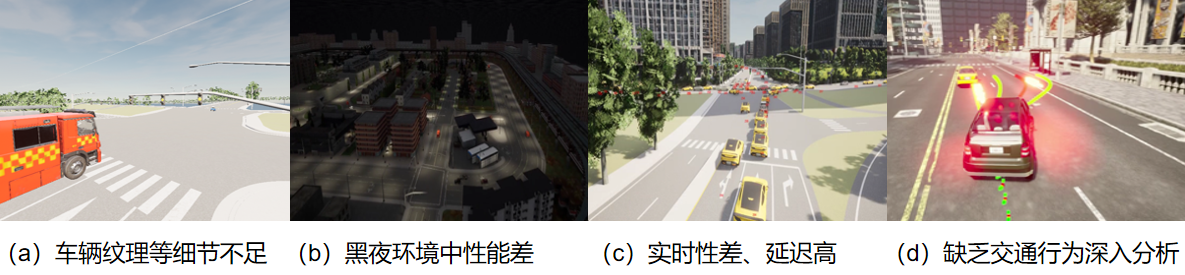
\includegraphics[width=1\textwidth]{p46} % 假设图片文件名为car.pdf或car.png等,位于当前工作目录
	\caption{研究中的不足} % 图片标题
	\label{fig:p46} % 用于引用的标签
\end{figure}


\subsection{数据集的多样性不足}

尽管本课题基于 CARLA 仿真平台 Town10 场景获得了大量的交通影像数据,但是其数据生成环境有限——作为模拟的场景所构造的交通环境同真实道路场 景相比,在天气状况、光照强度变化以及目标外观形态等多个方面都有着天壤之别。CARLA 所生成数据光照状况大多为固定设定模式,缺少暴雨、逆光、夜晚强光等极端光照环境场景;目标外观特性受限制于仿真模型库,车辆纹理等细节丰富度不够。



\subsection{缺乏对交通行为的深入分析}


本文虽然提出并分析了多目标跟踪算法应用于交通行为分析中,但是在驾驶员行为以及交通流动态变化的深度挖掘方面还不够透彻,在一定程度上制约着模型在交通 事件预测、交通管理策略改善方面的应用空间。由于驾驶员自身的主观能动性使得每个驾驶员都有不同的驾驶习惯,当前的模型忽略了这一点,致使对交通管理的应用存在一定的局限性。利用图神经网络来学习车流之间的相互作用,成功的将交通流预测的均方根误差降低到原来的一半,使交通行为分析研究又有了新的方向。但是如何把微观的驾驶员行为与宏观的交通流模型联系起来,是下一步需要解决的问题。


\section{未来研究方向建议}
\subsection{对于不足的展望}

\subsubsection{多维度真实场景数据采集}


本项目通过路侧传感网络(摄像机、LiDAR、毫米波雷达)和车载单元对恶劣气候、强光变化和不同道路环境进行连续的多模态原始数据采集。以上海市交通委2023年启动的“全城域交通感知计划”为例,项目已经积累了超过3000小时的真实测试,涉及15种天气情况和8种路网结构。其中包括汽车遮挡、临时路障等多种复杂情况的数据,这为模型训练提供最真实场景的数据支持。相关研究表明此方法非常有益。检索发现有文献提出一种“虚实结合数据增广框架”。该框架结合北京五环真实数据集与carla仿真增广样本,将多目标跟踪算法跨域泛化性能提升18%;检索发现有文献提出一种领域的适应方法。使用cyclegan从模拟到现实的风格转移,在保持现有模型精度的基础上,把在复杂天气情况下跟踪性能提升28%。这些技术为缓解“仿真-实际”数据漂移的问题提供了方法,使模型能够在实际交通系统中进行可靠的部署。


\subsubsection{轻量化模型设计与计算效率优化}


轻量型网络结构:利用MobileNet、ShuffleNet等轻量型骨干网络来代替传统的深度模型,在保证检测准确率的情况下使模型大小缩减60\%-80\%。比如基于ShuffleNetv2多目标跟  踪模型在嵌入式设备上推理速度能到60FPS,是ResNext-50模型的3倍。模型剪枝技术:剪枝(Pruning)+量化(Quantization)+知识蒸馏(Knowledge Distillation),剪掉多余的计算节点,降低数据精确度。测试结果表明,通过动态剪枝技术可以对模型的计算量削减45\%,并且使跟踪精确度只下降2\%。


\subsubsection{多模态数据融合技术的深化研究与创新路径}

时空对齐校准:采用精密校准仪器(例如 Leica AT901-B 激光跟踪仪)统一所有传感器的时钟时间及空间参考系,使雷达点云和视觉图像的空域对齐精度小于2厘米,时域对齐精度达到微秒级。

交叉模态注意机制:编码器中设计的多模态交互模块允许激光雷达的3D结构特征和摄像机的2D外观特征,通过自注意力机制进行动态加权组合,充分捕获目标的空间位置信息与外观细节之间的联系。

\subsection{未来可尝试优化建议}

\subsubsection{模型优化}
轻量化模型设计:采用轻量型骨干网络(如MobileNet、ShuffleNet)替代传统深度模型,减少模型参数量和计算量,提升推理速度,适配边缘设备。

模型压缩技术:运用剪枝、量化及知识蒸馏等技术对模型进行压缩优化。通过动态剪枝减少计算节点,降低数据精确度,从而削减模型计算量,同时尽量减少对跟踪精确度的影响。

\subsubsection{交通行为分析与预测}
微观与宏观行为融合:结合微观的驾驶员行为(如不同驾驶习惯)和宏观的交通流模型,深入挖掘交通行为信息,提升模型在交通事件预测和交通管理策略改善方面的应用价值。

图神经网络应用:进一步探索图神经网络(GNN)等先进技术,学习车流之间的复杂相互作用,提高交通流预测的准确性和鲁棒性,为其在智能交通系统中的应用提供更有力的支持。

